% Options for packages loaded elsewhere
\PassOptionsToPackage{unicode}{hyperref}
\PassOptionsToPackage{hyphens}{url}
%
\documentclass{article}
\usepackage{lmodern}
\usepackage{hyperref}
\usepackage{amssymb,amsmath}
\usepackage{ifxetex,ifluatex}
\usepackage{amssymb}
\usepackage{cite}
\usepackage{listings}
\usepackage{float}
\usepackage{subfig}
\usepackage{color}
\usepackage{amsmath}
\setcounter{tocdepth}{3}
\usepackage{graphicx}
\usepackage{amssymb}
\usepackage[a4paper]{geometry}
\usepackage[T1]{fontenc}
\usepackage{color}
\usepackage{url}
\usepackage[dvipsnames]{xcolor}
\usepackage{hyperref}
\hypersetup{
    colorlinks=true,
    linkcolor=violet,
    filecolor=magenta,      
    citecolor=blue,
    urlcolor=cyan,
}
\usepackage{graphicx}
\usepackage{mathtools}

\DeclarePairedDelimiter\ceil{\lceil}{\rceil}
\DeclareMathOperator*{\argmin}{argmin}
\DeclarePairedDelimiter\floor{\lfloor}{\rfloor}


\newcommand{\wek}[1]{
	{\bf{#1}} 
}
\newcommand{\jed}[1]{
	{$\left[#1\right]$}
}
\newcommand{\mat}[1]{
	{\bf #1} 
}
\newcommand{\todo}[1]{
	\colorbox{yellow} {{\color{red}
	\emph {TODO: #1}
}}}
\newcommand{\srednia}[1]{
	\langle #1 \rangle 
}




\title{Analiza metod detekcji anomalii na podstawie przebiegu kursów
instrumentów finansowych}
\author{Aleksandra Dzieniszewska \and Eryk Warchulski}
\date{}

\begin{document}
\maketitle
\begin{abstract}
  Celem niniejszego dokumentu jest przedstawienie wstępnych założeń
  dotyczących realizacji projektu analizy algorytmów detekcji anomalii w
  szeregach czasowych, tj. TSAD (z ang. \textbf{time series anomaly
  detection}). W jego ramach zostanie omówiona domena problemu, tj.
  przebiegi wartości instrumentów finansowych na różnych typach rynków,
  model zjawiska detekcji anomalii oraz plan eksperymentów. Opisane
  zostaną również metryki jakości uzyskiwanych rozwiązań jak i źródło
  pozyskiwanych danych.
\end{abstract}

\section{Wprowadzenie}


  Przebieg kursów aktywów finansowych jak na przykład kursów akcji
  spółek lub indeksów giełdowych jest fundamentem działania inwestorów na
  rynkach. Jego zachowanie determinuje strategie oraz ryzyko inwestycyjne.
  W związku z powyższym  kursy akcji są szczególnie interesujące nie
  tylko dla bezpośrednich aktorów rynkowych, ale również ekonomistów lub
  statystyków, którzy opracowują modele zachowań tych kursów lub rynków w
  ogólności. Współcześnie bardzo dużo uwagi poświęca się zagadnieniom
  predykcji przyszłych wartości kursów, co stanowi złożony i trudny
  problem, biorąc pod uwagę fakt, że jedna z dominujących teorii
  rynkowych, tj. EFM (z ang. \textbf{efficient-market hypothesis}) uważa
  za niemożliwe dokonywanie przydatnych predykcji \cite{RandomWalk}
  przyszłych kursów, a ponadto uznaje się, że rynki finansowe nie są
  obojętne na predykcje jak np. pogoda \cite{Sapiens}. Niemniej jednak
  problem predykcji przyszłych wartości kursów nie jest jedynym
  zagadnieniem, które ma praktyczne znaczenie. Możliwość odróżnienia
  niestandardowych fluktuacji kursów i tym samym punktów odstających może
  stanowić istotną informację dla inwestorów i zaangażować dedykowane
  takim zdarzeniom procesy biznesowe. Szczególnie istotne wydaje się to z
  punktu widzenia zautomatyzowanych rynków giełdowych, w których akcje
  podejmowane przez aktorów (systemy decyzyjne) mierzone są w
  milisekundach, a dane giełdowe mogą być traktowane jako strumieniowe
  \cite{HFT-wiki}. Wówczas wykrycie anomalii i jej odpowiednie obsłużenie
  wydaje się być krytyczne dla gracza rynkowego.
  \newline
  Dalszy rozkład dokumentu jest następujący: w rodziale drugim (\ref{r2}) krótko
  scharakteryzowane są wielkości, których przebieg zostanie poddany baddaniu w ramach projektu. Rodział (\ref{r3}) definiuje podstawowe pojęcia związane z zadaniem detekcji anomalii. W rozdziale (\ref{r4}) zarysowane są idee, które stoją za stosowanymi przez autorów algorytmami. Rozdział (\ref{r5}) i (\ref{r6}) zawierają kolejno -- opis danych, które bedą stosowane, oraz plan eksperymentów. 

  \section{Rynki finansowe \label{r2}}

  W ramach realizacji projektu użyte zostaną łącznie dwa zbiory danych, na
  które składają się przebiegi kursów instrumentów finansowych. Jeden z
  nich będzie pochodzić z rzeczywistego rynku finansowego, a drugi z rynku
  wirtualnego. Motywacją takiego podejścia jest chęć zaobserwowania
  zachowania się rynku w świecie, w którym na wartość kursu wpływa bardzo
  duża liczba czynników jawnych lub niejawnych, oraz w świecie, w którym
  zbiór możliwych akcji podejmowanych przez aktorów jest znacząco
  ograniczony oraz sam świat ma raczej charakter statyczny i iteracyjny.
  Ponadto dodatkową motywacją za skorzystaniem z danych pochodzących z
  rynku wirtualnego jest łatwość określenia zdarzeń, które powodują nagłe
  zmiany przebiegu kursu -- co zostanie bardziej szczegółowo opisane w
  podsekcji poświęconej temu rynkowi.

\subsection{Rynki rzeczywiste}

  \emph{Indeks giełdowy WIG20} jest statystyką (średnia ważona
  kapitalizacją spółek) obrazującą zmianę cen akcji dwudziestu
  największych spółek akcyjnych notowanych na Warszawskiej Giełdzie
  Papierów Wartościowych. Wartość indeksu pozwala ocenić inwestorom ogólny
  kierunek zmian cen i stan rynku.

  Przebieg indeksu WIG20 w wybranym przedziale czasowym pokazany jest na
  rysunku poniżej.

\begin{figure}
    \centering
    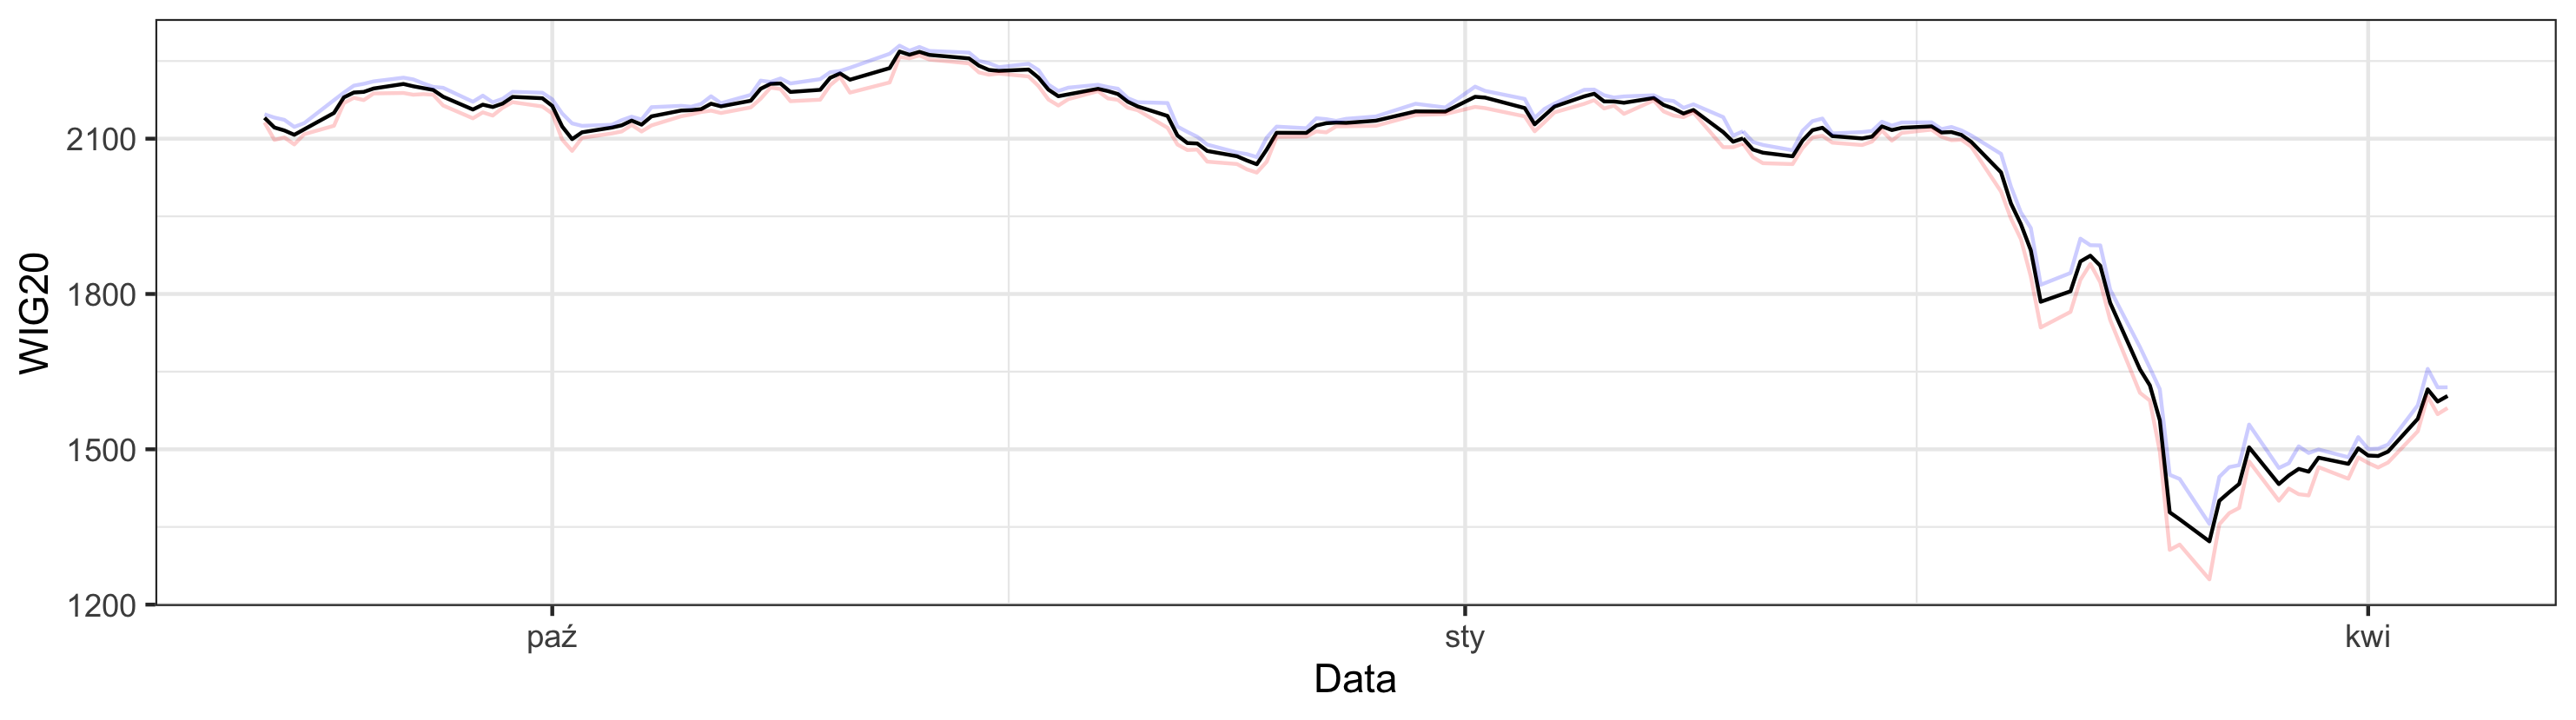
\includegraphics[width=\textwidth]{./images/wig20-random.png}
    \caption{Przebieg indeksu giełdowego WIG20. Rysunek własny.}
\end{figure}
\subsection{Rynki wirtualne}

\emph{WoW Token} jest przedmiotem w grze MMO-RPG (\emph{Massively
multiplayer online role-playing game}) \emph{World of Warcraft}, który
przez gracza może zostać wykorzystany w następujące sposoby:

\begin{itemize}
\item
  gracz może kupić token za rzeczywistą walutę (USD, GBP, EUR, TWD,
  KRW), a następnie sprzedać go w umieszczonym w grze domu aukcyjnym
  (\emph{Auction House})
\item
  gracz może kupić token, płacąc fikcyjną walutą obowiązującą w świecie
  \emph{World of Warcraft} (dalej G), a następnie wymienić go na
  przedłużenie abonamentu gry lub wymienić go na bon w internetowym
  sklepie wydawcy gry.
\end{itemize}

Kurs wymiany G/USD jest stały i wynosi $20$ \footnote{To samo tyczy
  się jakiejkolwiek innej waluty rzeczywistej.} natomiast kurs tokena w
świecie gry jest zmienny i zależy głównie od podaży i popytu
\cite{wtoken-info}.

Przebieg ceny tokena w grze na serwerach europejskich w wybranym czasie
jest pokazany na poniższym rysunku.

\begin{figure}
  \centering
  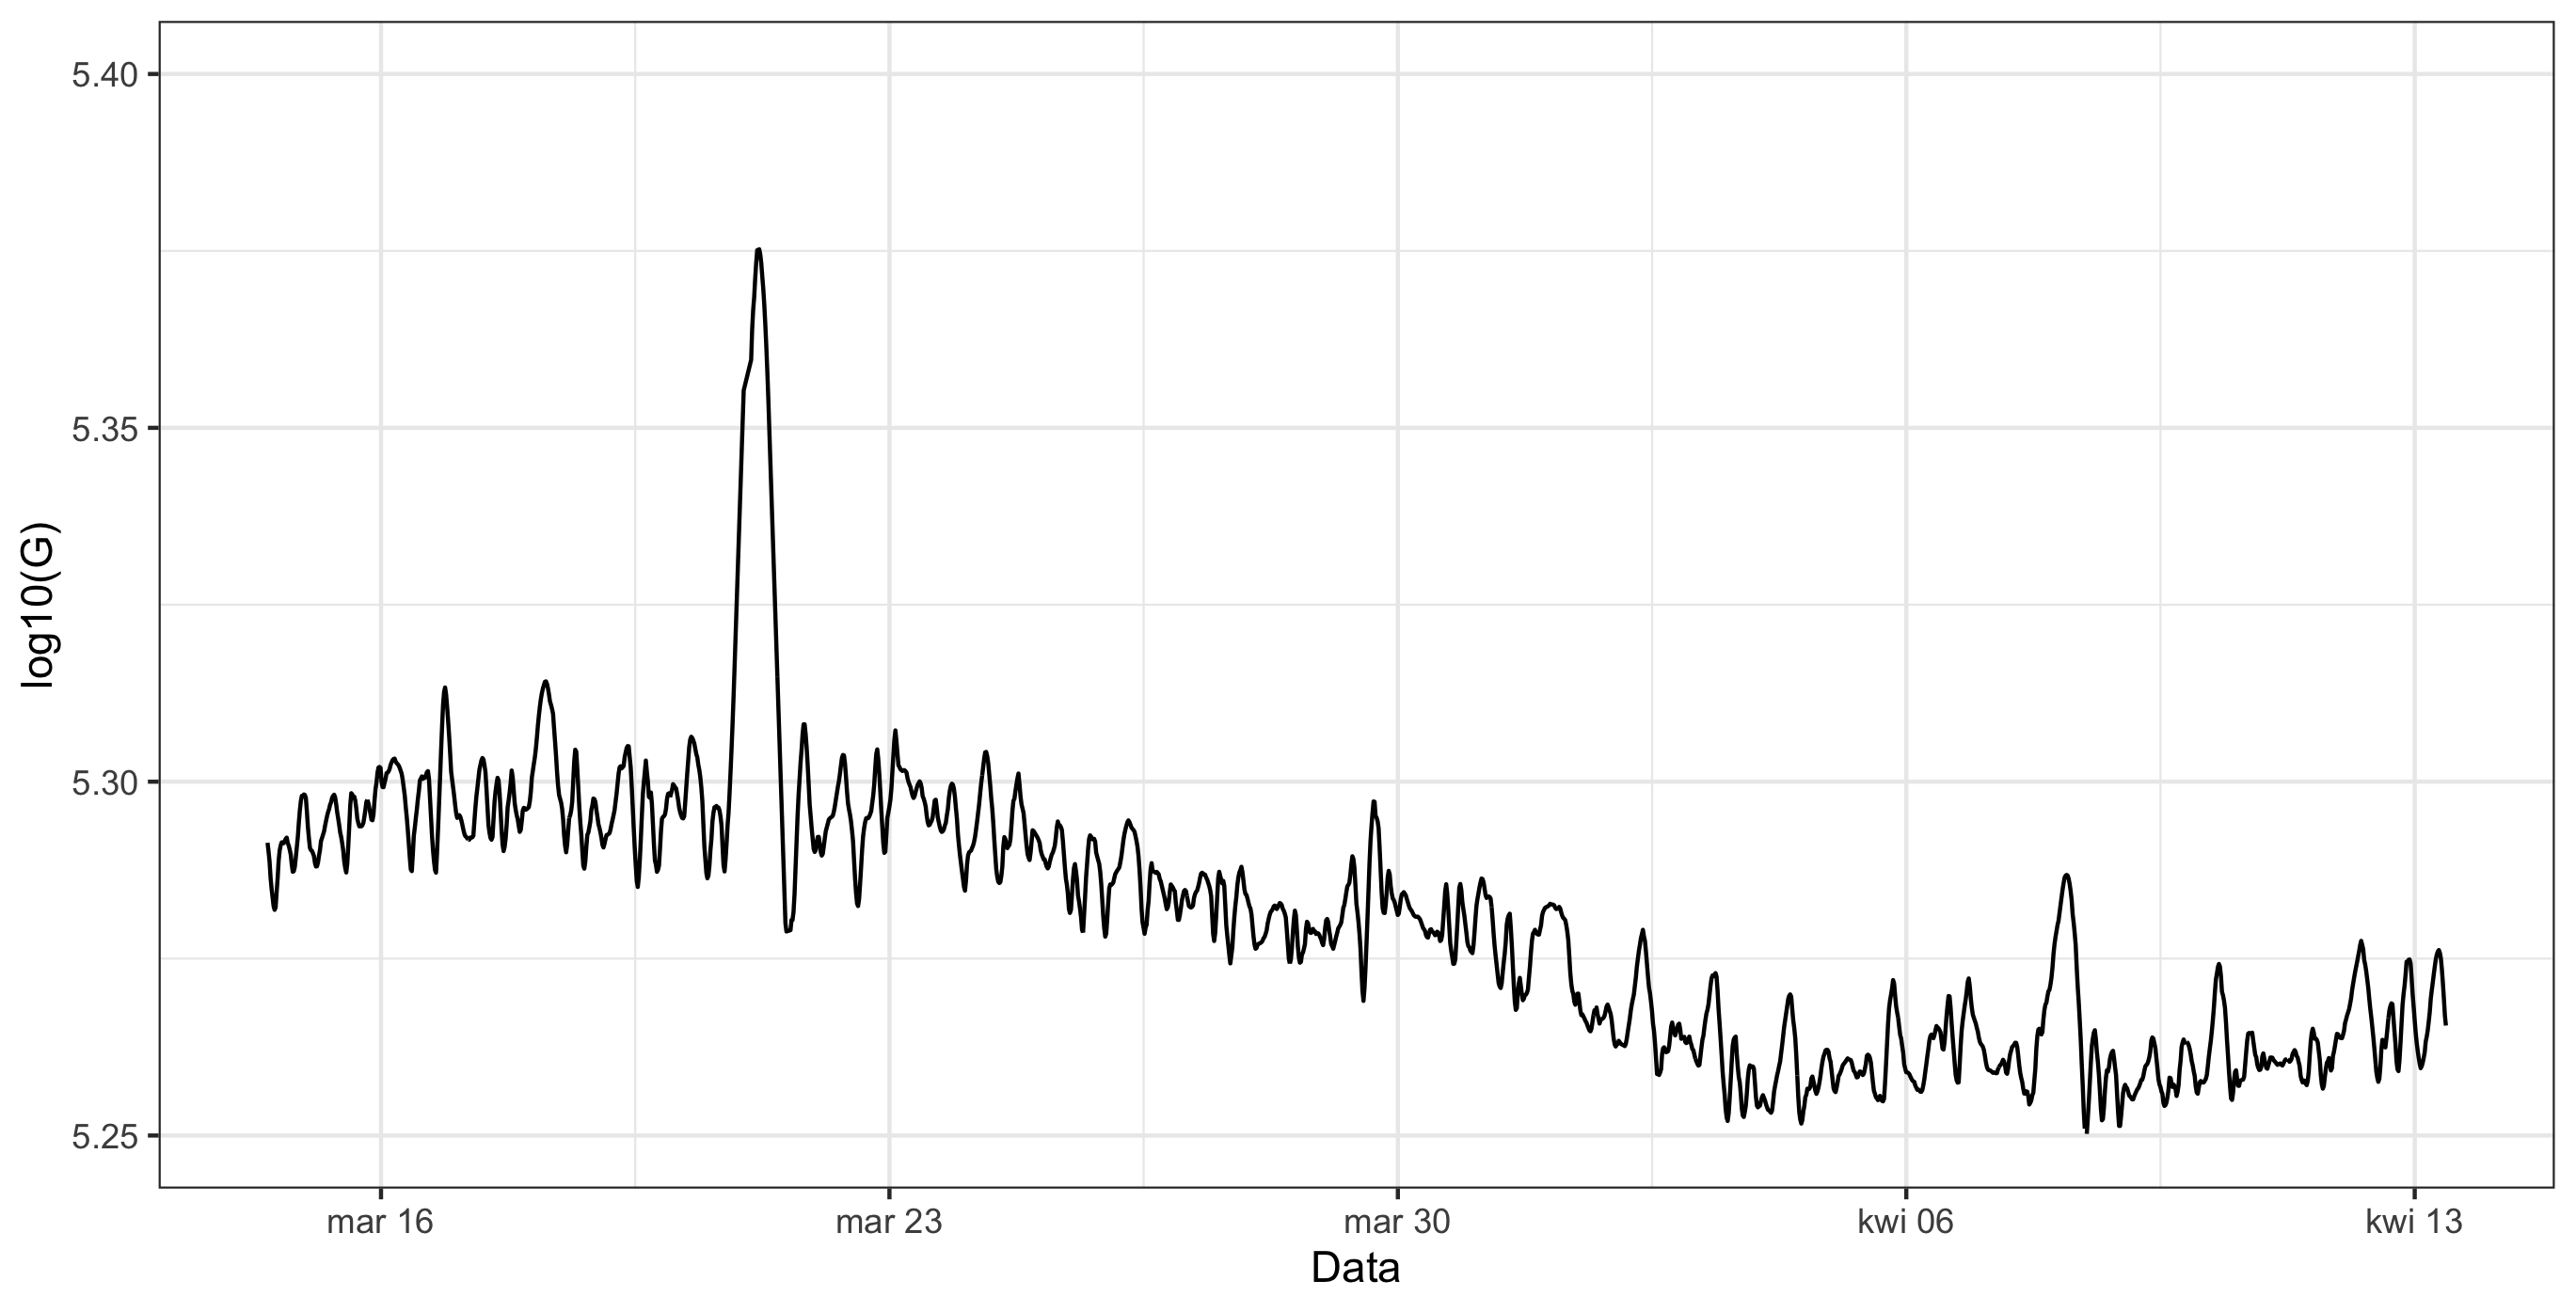
\includegraphics[width=\textwidth]{./images/wtoken-random.png}
  \caption{Przebieg wartości WoW tokna. Rysunek własny.}
\end{figure}

\section{Zadanie detekcji anomalii \label{r3}}

W rozdziale tym zostanie zdefiniowany w ogólny sposób problem detekcji
anomalii w szeregach czasowych. Konkretyzacja ogólnych pojęć
zdefiniowanych poniżej zostanie przedstawiona w rozdziale dotyczącym
algorytmów detekcji.

Przez zadanie detekcji anomalii w trakcie realizacji projektu będziemy
rozumieć następujący problem:

\begin{description}
\item[Szereg czasowy]
niech \((X_{i})_{i \in T}\) będzie procesem stochastycznym określonym na
pewnej przestrzeni probabilistycznej, a zbiór indeksów \(T\) będzie
interpretowany jako zbiór chwil czasowych jednakowo odległych od siebie.
Realizację tego procesu, tj. uporządkowany zbiór
\(\{x{_t}\}_{t = 1, \dots, N}\), będziemy nazywać szeregiem czasowym.
Nie zakładamy ponadto niczego względem stacjonarności tego szeregu lub
rozkładu prawdopodobieństwa, z którego jest on generowany poza faktem,
że jego nośnikiem jest zbiór liczb rzeczywistych \(\mathbb{R}\).
\item[Anomalia]
Anomalią w szeregu czasowym będziemy nazywali punkt w tym szeregu
\(x_{k}\), który według przyjętego kryterium \emph{odstaje} od
pozostałych punktów w najbliższym sąsiedztwie
\(x_{k - s}, \dots, x_{k + s}\) (anomalia lokalna) lub względem
wszystkich punktów w szeregu (anomalia globalna). Kryterium
\emph{odstawania} jest silnie zależne od kontekstu i procedury detekcji
anomalii. Często przyjmowane kryterium wygląda następująco
\cite{ad_review}:
\end{description}


\begin{equation}
  \label{eq1}
  |x_t - s(\{X_{t}\})| > \tau
\end{equation}

przy czym \(s(\star)\) jest pewną funkcją.

\begin{description}
\item[Detekcja anomalii]
Detekcją anomalii będziemy nazywali procedurę, pozwalającą wykryć w
    szeregu czasowym zbiór indeksów $T_{A}$ punktów uznawanych za anomalię:
\end{description}

\begin{equation*}
AD\colon \{X_{t}\} \rightarrow T_{A} \subset T.
\end{equation*}

\section{Algorytmy detekcji anomalii \label{r4}}

W rozdziale tym zostaną opisane algorytmy służące do detekcji anomalii,
które w ramach projektu zamierzamy zbadać. Opis ten nie będzie zawierał
dokładnego pseudokodu, a jedynie pewien formalizm matematyczny, który
pozwala zobrazować idee stojące za omawianymi metodami. Ponadto wskazane
i omówione zostaną parametry tych metod.

Omawiane metody

\subsection{MAD}

Metoda \emph{MAD}, tj. \emph{median absolute deviation} jest stosunkowo
prostym sposobem detekcji anomalii opartym na oknie kroczącym (z ang.
\emph{moving window}) o długości \(k\). Dla każdego punktu metoda estymuje
dwie wielkości:

\begin{enumerate}
\item
  medianę w oknie
\item
  bezwzględne odchylenie mediany.
\end{enumerate}


Model można sformalizować w następujący sposób:
dla każdego punktu szeregu czasowego \(x_{i}\) liczona jest wielkość

\begin{equation*}
MAD_{i} = median_{i}[x_{i} - median_{j}(x_{j})].
\end{equation*}

przy czym $median_{j}(\star)$ jest medianą $j$-tego okna.

Następnie każdy punkt szeregu czasowego porównywany jest z odpowiadającą
mu wartość \(MAD_{\star}\) -- jeśli wartość bezwzględna różnicy między
tym punktem, a wartością \(MAD\) jest większa od ustalonego progu, to
punkt jest klasyfikowany jako anomalia. W nawiązaniu do (\ref{eq1}) -- kryterium
konkretyzuje się do postaci:

\begin{equation*}
|x_{t} - MAD_{t}| > \tau.
\end{equation*}

\hypertarget{stl-esd}{%
\subsection{STL-ESD}\label{stl-esd}}

Metoda STL (z ang. \emph{Seasonal-Trend decomposition using Loess})
opiera się na dekompozycji addytywnej szeregu czasowego na trzy składowe
w następującej formie

\begin{equation*}
x_{t} = \tau_{t} + s_{t} + r_{t},\; t = 1, \dots, N
\end{equation*}



gdzie \(x_{t}\) jest obserwowaną wartością szeregu czasowego,
\(\tau_{t}\) jest składową trendu, \(s_{t}\) składową sezonowości, a
\(r_{t}\) składową rezyduów. Dekompozycja taka jest dedykowana szeregom
czasowym z zauważalnymi wolnozmiennymi fluktuacjami sezonowości oraz
szybkozmienną składową trendu \cite{wen-gao}. Zakłada się
ponadto, że składowa rezyduów zawiera całą pozostałą informację o
szeregu czasowym -- m.in. szum. Można to sformalizować w następujący
sposób:

\begin{equation*}
  r_{t} = a_{t} + \epsilon_{t}
\end{equation*}



przy czym składowa \(\epsilon_{t}\) jest składową szumu, a \(a_{t}\)
modeluje poszukiwane anomalie w postaci nagłych przyrostów wartości
(t.zw. \emph{peak}'ów). Dekompozycja STL jest procedurą iteracyjną i
szczegółowo zostanie opisana w dokumentacji końcowej projektu. Na
potrzeby tego dokumentu należy zaznaczyć, że wynikiem dekompozycji jest
składowa \(a_{t}\), a składowa:

\begin{itemize}
\item
  szumu \(\epsilon_{t}\) jest usuwana wskutek operacji filtracji (ang.
  \emph{denoising}) przy pomocy średniej/mediany kroczącej lub
  probabilistycznemu wygładzaniu eksponencjalnego (PEWMA) \cite{PEWMA}
\item
  trendu \(\tau_{t}\) jest usuwana wskutek operacji detrendyzacji, która
  w najprostszym wariancie sprowadza się do zastosowania operatora
  różnicowego \begin{equation*} \nabla x_{t} = x_{t} - x_{t -1} \end{equation*}
    lub do filtrów kroczących
\item
  sezonowości \(s_{t}\), która jest usuwana w standardowej wersji
  metody STL przy pomocy LOESS (ang. \emph{locally estimated scatterplot
  smoothing}), tj. metody łączącej działanie średniej kroczącej z
  regresją wielomianową \cite{stl-origin}.
\end{itemize}

STL zawiera trzy parametry sterujące metodą:

\begin{enumerate}
\def\labelenumi{\arabic{enumi}.}
\item
  \(n_{p}\) liczbę obserwacji, która jest rozważana w każdym cyklu
  wyliczania składowej sezonowości
\item
  \(n_{i}\) liczbę iteracji wewnętrznej pętli algorytmu
\item
  \(n_{o}\) liczbę iteracji pętli zewnętrznej
\end{enumerate}

oraz trzy lub więcej parametrów sterujących detrendyzacją, usunięciem
szumu oraz ekstrakcją sezonowości.

Po otrzymaniu składowej \(a_{t}\) stosowany jest test statystyczny ESD
(z ang. \_Extreme Studentized Deviate), który służy do wykrycia
anomalii w próbie o rozkładzie \emph{asymptotycznie} normalnym. Jest on
uogólnieniem testu Grubbs'a, w którym rozkład normalny próby jest
warunkiem koniecznym. Test ESD rozważa dwie hipotezy

\newtheorem{nullhypothesis}{$H_0\colon$}
\newtheorem{althypothesis}{$H_1\colon$}

\begin{nullhypothesis}
  w próbie \(\{a_1, \dots, a_{n}\}\) nie ma punktów odstających (anomalii) 
\end{nullhypothesis}

\begin{althypothesis} 
  w próbie \(\{a_1, \dots, a_{n}\}\) jest co najwyżej \(K\) punktów odstających.
\end{althypothesis}


\(i\)-ta statystyka testowa ESD wyliczana jest w następujący sposób:

\begin{equation*}
T^{ESD}_{i} = \frac{\max_{i}|a_{i} - \bar a|}{\sigma}
\end{equation*}

gdzie \(\bar{a}\) oznacza średnią z próby, a \(\sigma\) odchylenie
standardowe z próby. Po wyliczeniu \(T^{ESD}_{i}\) usuwana jest z próby
obserwacja maksymalizująca licznik i liczona jest kolejna statystyka
testowa na podstawie zmodyfikowanej próby.

Po wyliczeniu \(\{T^{ESD}_{i}\}_{i = 1, \dots, K}\) wyliczane są
wartości krytyczne testu \(\lambda_{i}\) będące funkcją rozkładu
t-studenta z \(N - i\) stopniami swobody.

Liczbę anomalii w próbie znajduje się przez podanie największego \(i\)
takiego, że \(T^{ESD}_{i} > \lambda_{i}\).

W kontekście definicji procedury detekcji anomalii podanej (\ref{r3})
należy wybrać z próby \(i\) największych elementów i ich znaczniki
umieścić w zbiorze \(T_{A}\).

Dekompozycja szeregu czasowego przez algorytm STL znajduje się na
poniższym obrazku.

\begin{figure}
\centering
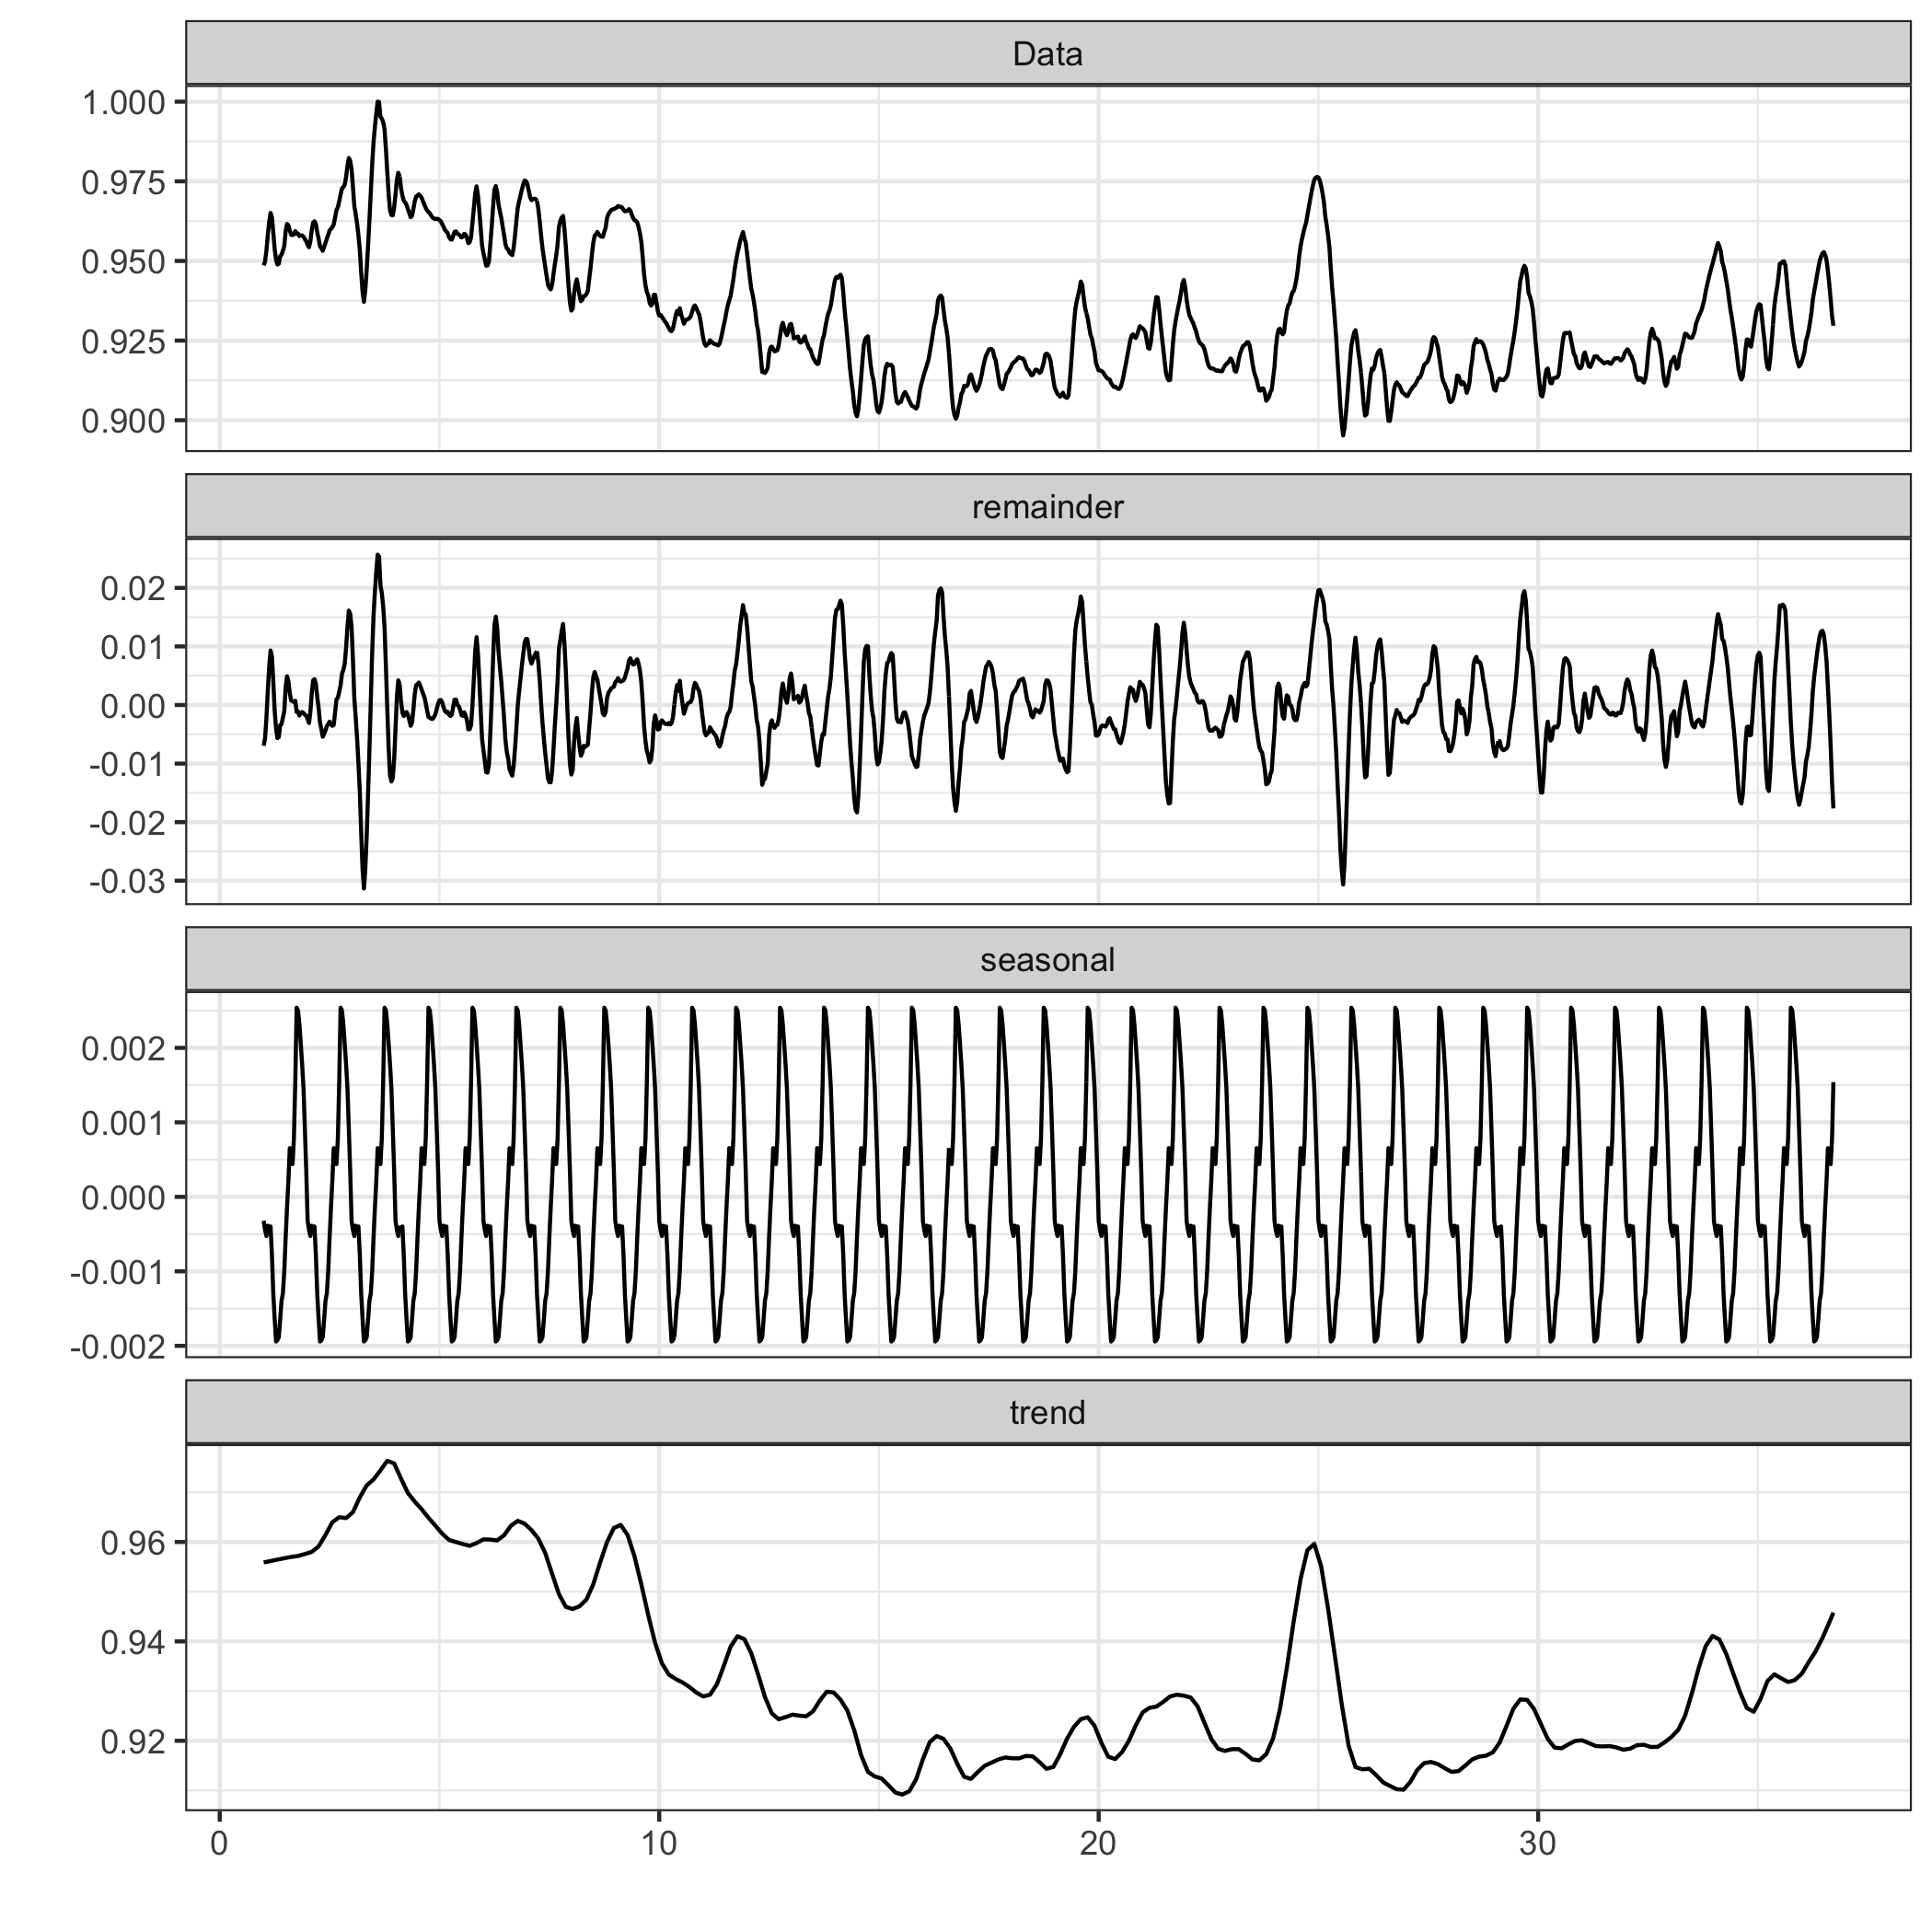
\includegraphics[width=\textwidth]{./images/stl-usage.png}
\caption{Dekompozycja szeregu czasowego metodą STL. Rysunek własny.}
\end{figure}

\subsection{LDCD}

Metoda LDCD  (z ang. \emph{Lazy Drifting Conformal Detector}) \cite{knn} jest procedurą detekcji anomalii opartą
na algorytmie $k$-NN, która nie czyni żadnych założeń odnośnie rozkładu szeregu czasowego i jego właściwości.

Algorytm bazuje na kroczącym oknie historii o długości $l$, które zanurza (ang. \emph{embed}) szereg czasowy w przestrzeni $l$-wymiarowej.
Operacja taka umożliwia zastosowanie metod wielowymiarowych do przyporządkowania punktom szeregu czasowego punktów niedopasowania (z ang. \emph{non-conformity score}) $\alpha_{t}$. Punkty te są przyznawane w oparciu o metodę $k$-NN. 
Metoda ta ponadto utrzymuje w trakcie swojego działa dwa zbiory:

\begin{itemize}

  \item zbiór referencyjny $T_{t}$ o wielkości $n$
  \item zbiór korekcyjny $A_{t}$ o wielkości $m$ 

\end{itemize}

przy czym $t \geq m+n$. Znaczenie obu struktur i dokładne działanie algorytmu zostanie omówione w dokumetancji końcowej.


\section{Charakterystyka zbioró wdanych \label{r5}}

Zbiory danych użyte do analizy działania algorytmów zostały częściowo
omówione w rozdziale \ref{r2}. W niniejszym rozdziale zostaną wskazane
źródła, z których pochodzą dane, oraz podana zostanie krótka
charakterystyka tych danych.

Kompletna analiza statystyczna danych, na którą będzie składało się
zbadanie rozkładu danych, autokorelacji szeregu czasowego lub jego
innych właściwości jak stacjonarność zostanie umieszczona w dokumentacji
końcowej.

\subsection{WIG20}

Historyczne dane \texttt{WIG20} dostępne są do pobrania ze strony
\href{https://stooq.pl/q/d/?s=wig20}{stooq.pl} z interwałem:

\begin{itemize}
\item
  dziennym
\item
  tygodniowym
\item
  miesięcznym
\item
  kwartalnym
\item
  rocznym.
\end{itemize}

Dane pobierane są w formacie \texttt{CSV} i nie zawierają wartości
brakujących. Struktura zbioru danych przedstawiona jest na poniższym
obrazku.

\begin{figure}[H]
  \centering
  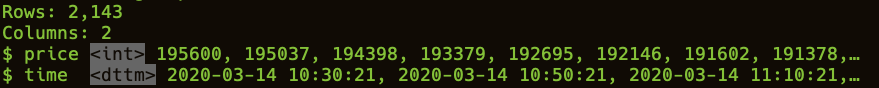
\includegraphics[width=.75\textwidth]{./images/wt-glimpse.png}
  \caption{Wynik wypisania na konsolę fragmentu zbioru danych.}
\end{figure}

Należy jednak zaznaczyć, że rozważaną w projekcie wartością szeregu
czasowego jest uśredniona wartość indeksu z wartości otwarcia,
zamknięcia oraz wartości najmniejszej i największej danej sesji.

Wartości indeksu WIG20 dostępne są od 16 kwietnia 1991 do dnia
dzisiejszego (02.04.2020) z tą uwagą, że nie we wszystkich przypadkach
zachowany jest wymagany interwał, co jest zaznaczone na rysunku poniżej.

\begin{figure}[H]
  \centering
  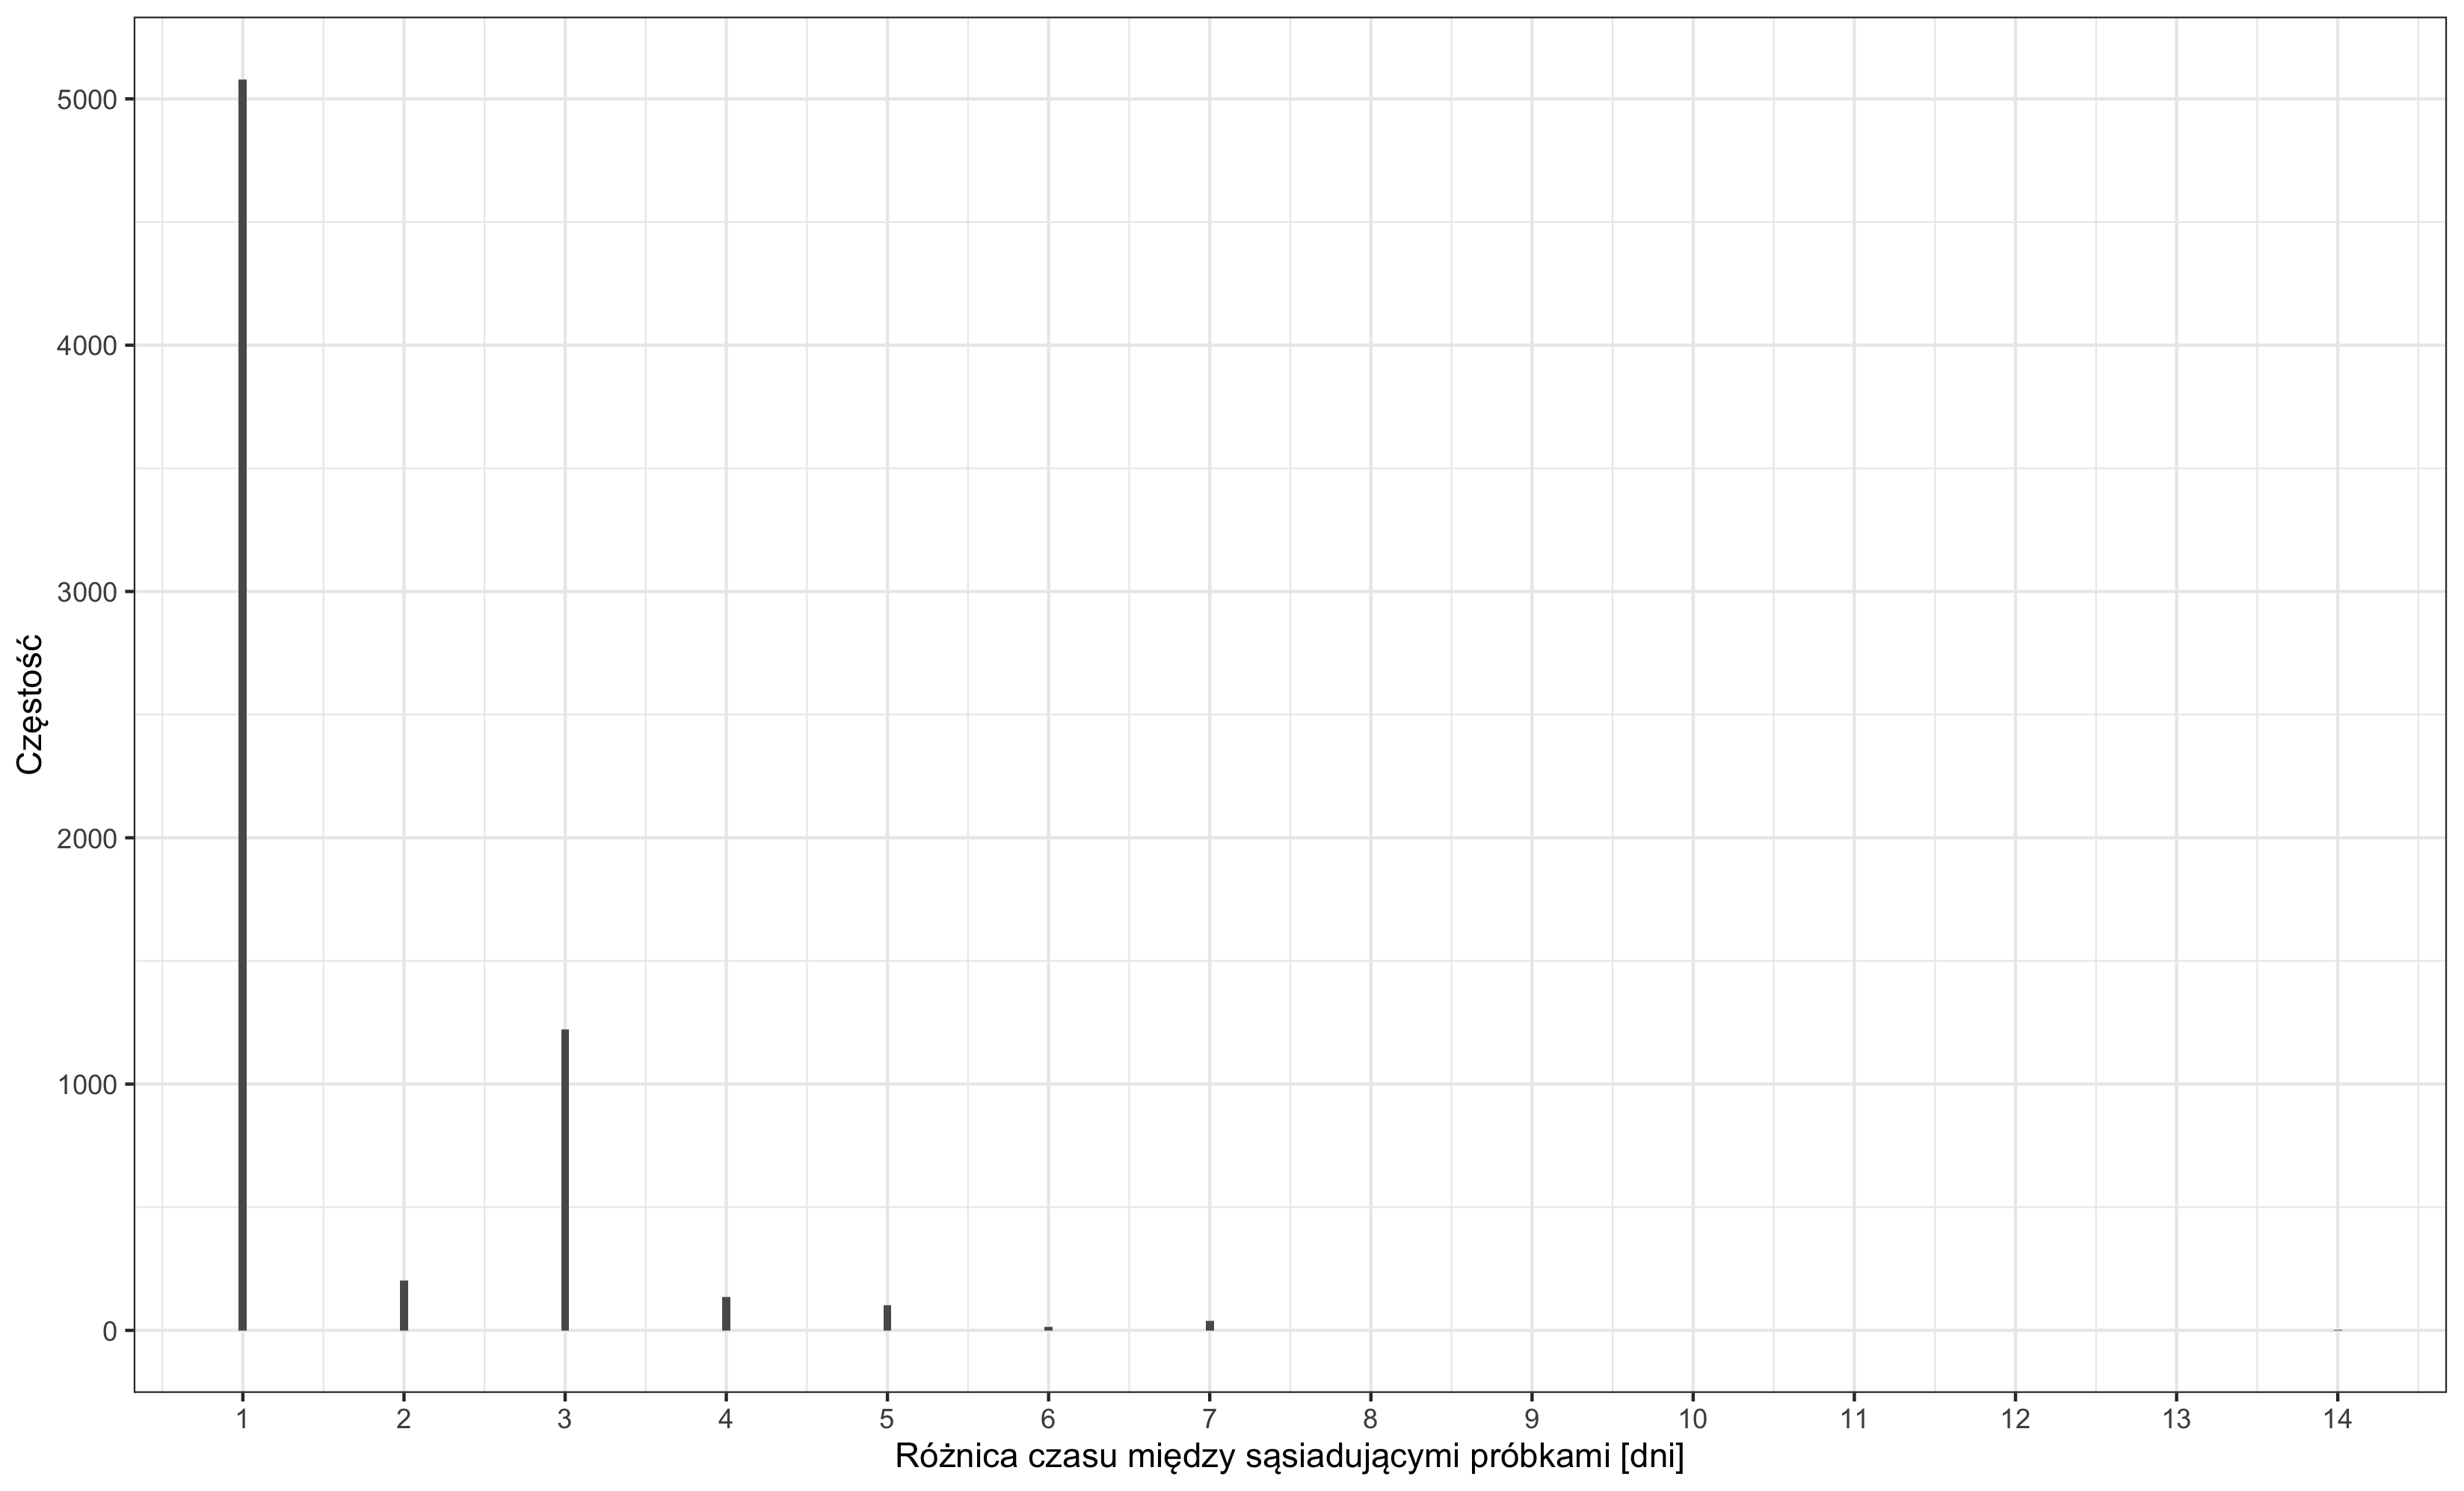
\includegraphics[width=.75\textwidth]{./images/tdiff.png}
  \caption{Histogram odstępów między sąsiadującymi próbkami w zbiorze danych WIG20. Rysunek własny.}
\end{figure}

W związku z tym do badań zostanie użyty najdłuższy podciąg, w którym
odstęp między danymi wynosi jedną dobę.

\hypertarget{wow-token}{%
\subsection{WoW Token}\label{wow-token}}

Historyczne kursy tokena dostępne są na stronie
\href{https://wowtokenprices.com/}{wowtokenprices.com}. Serwis
udostępnia API, które umożliwia pobrania danych z kwantem 20-minutowym,
które nie zawierają wartości brakujących, od początku istnienia tokena,
tj. od roku 2015. Kurs tokena różni się między regionami, w których
znajdują się serwery. Dostępnych jest 5 regionów, tj.

\begin{enumerate}
\def\labelenumi{\arabic{enumi}.}
\item
  europejski
\item
  amerykański
\item
  chiński
\item
  tajwański
\item
  koreański.
\end{enumerate}

Struktura zbioru danych z ostatniego miesiąca widoczna jest na na
poniższym obrazku.

\begin{figure}[H]
  \centering
  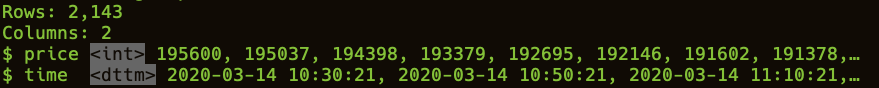
\includegraphics[width=.75\textwidth]{./images/wt-glimpse.png}
  \caption{Wynik wypisania na konsolę fragmentu zbioru danych.}
\end{figure}


\section{Plan badań \label{r6}}

Celem projektu jest zbadanie i porównanie metod detekcji anomalii w
szeregach czasowych przy pomocy danych scharakteryzowanych we
wcześniejszych rozdziałach.

Przyjęta metodologia zakłada, że zadanie detekcji anomalii zostanie
potraktowane jak zadanie klasyfikacji binarnej. Oznacza to, że przykłady
w zbiorze danych zostaną oznaczone flagą, która informuje o tym czy dany
przykład jest anomalią czy też nie.

Przydział flagi będzie odbywał się na dwa sposoby:

\begin{enumerate}
\def\labelenumi{\arabic{enumi}.}
\item
  autorzy manualnie wybiorą podzbiór zdarzeń, których zajście
  spowodowało znaczny przyrost lub spadek wartości indeksu/tokena i
  oznaczą je jako anomalie. Przykłady takich zdarzeń są następujące:
\end{enumerate}

\begin{itemize}
  \item kryzys gospodarczy z 2008 roku (ogłoszenie upadłości przez bank \emph{Lehman Brothers}) (WIG20)
\item rozpoczęcie stanu epidemicznego w Polsce w związku z pandemią koronawirusa SARS-CoV-2 (WIG20)
\item atak Iranu na bazy wojskowe USA na początku 2020 roku (WIG20)
\item zwiększenie współczynnika przyrostu zdobywanego doświadczenia o $100 \%$ (WoW Token)
\item wydanie nowej części gry \emph{World of Warcraft} (WoW Token).
\end{itemize}

\begin{enumerate}
\def\labelenumi{\arabic{enumi}.}
\setcounter{enumi}{1}
\item
  do zbiorów danych zostaną wprowadzone anomalie w sposób losowy.
\end{enumerate}

Dzięki takiemu podejściu możliwe będzie porównanie metod detekcji w dość
ogólnym kontekście (dane równie dobrze mogłyby być syntetycznie
generowane) oraz sprawdzenie jak metody radzą sobie z wykrywaniem
anomalii, które odpowiadają przełomowym zdarzeniom i mają
odzwierciedlenie na rynkach. Przyjęcie takiej metodologii podyktowane jest faktem, że w dostepnych zbiorach danych autorom nie udało się znaleźć zbioru poświęconemu aktywom giełdowym.

Porównanie modeli odbędzie się przy pomocy trzech miar:

\begin{enumerate}
\def\labelenumi{\arabic{enumi}.}
\item
  precyzji 
    \begin{equation*}
       P = \frac{|S \cap G|}{|S|}
    \end{equation*}
\item
  odzysku (z ang. \emph{recall}) 
    \begin{equation*}
      R = \frac{|S \cap G|}{|G|}
    \end{equation*}

\item
  miary $F-1$
    \begin{equation*}
    F = 2\frac{PR}{P + R}
    \end{equation*}
  będącej średnią harmoniczną \(P\) i \(R\)
\end{enumerate}

przy czym \(S\) jest zbiorem poprawnie rozpoznanych anomalii, a \(G\)
jest zbiorem wszystkich anomalii w zbiorze danych.

Ponadto zbadane zostaną różne nastawy parametrów sterujących użytych
metod jak:

\begin{itemize}
\item
  sposób dokonywania dekompozycji sygnału w metodzie STL

  \begin{itemize}
  \item
    zastąpienie składowej trendu medianą \cite{adts-cloud}
  \item
    użycie różnych metod usunięcia szumu, tj. np. SMA oraz PEWMA
  \end{itemize}
\item
  wpływ szerokości okna na działanie metody MAD
\item
  wpływ wielkości kolejki strojenia (\emph{calibration queue}), długości
  zbioru referencyjnego oraz parametru metody NN na działanie algorytmu
  CAD $k$-NN.
\end{itemize}

\bibliography{biblio} 
\bibliographystyle{ieeetr}
\end{document}
